\documentclass[aspectratio=169]{beamer}
\usetheme{Madrid}
\usepackage{booktabs}
\usepackage{graphicx}
\usepackage{array}

\title{Branch Specialization Checkpoint}
\subtitle{Toy Competition Weight Sweep}
\author{Branch Specialization Project}
\date{2026-05-22}

\begin{document}

\begin{frame}
  \titlepage
  \vspace{-0.5em}
  \begin{center}
    Checkpoint reason: the weight sweep gives a sharper mechanism for Phase 3.
  \end{center}
\end{frame}

\begin{frame}{Current Question}
  \textbf{Phase 3 RQ:} Does structural heterogeneity cause stable functional specialization?

  \vspace{0.9em}
  The layout-permutation result showed that the local role follows the 64-dim head,
  while induction is layout-sensitive.

  \vspace{0.9em}
  This checkpoint asks:

  \begin{quote}
    If local-task pressure is reduced, does induction reclaim the 64-dim slot?
  \end{quote}

  This directly tests capacity-slot competition.
\end{frame}

\begin{frame}{Experiment Setup}
  \begin{itemize}
    \item Layout: \texttt{hetero4\_64second = [16, 64, 16, 32]}.
    \item This was diagnostic because equal weights gave induction-on-64 in only 1/5 seeds.
    \item Induction weight fixed at 1.0.
    \item Local weight swept: 0.00, 0.01, 0.10, 0.25, 1.00.
    \item Five seeds per condition, 1200 training steps per seed.
    \item Role score is single-head causal ablation loss delta.
  \end{itemize}
\end{frame}

\begin{frame}{Main Evidence}
  \begin{center}
  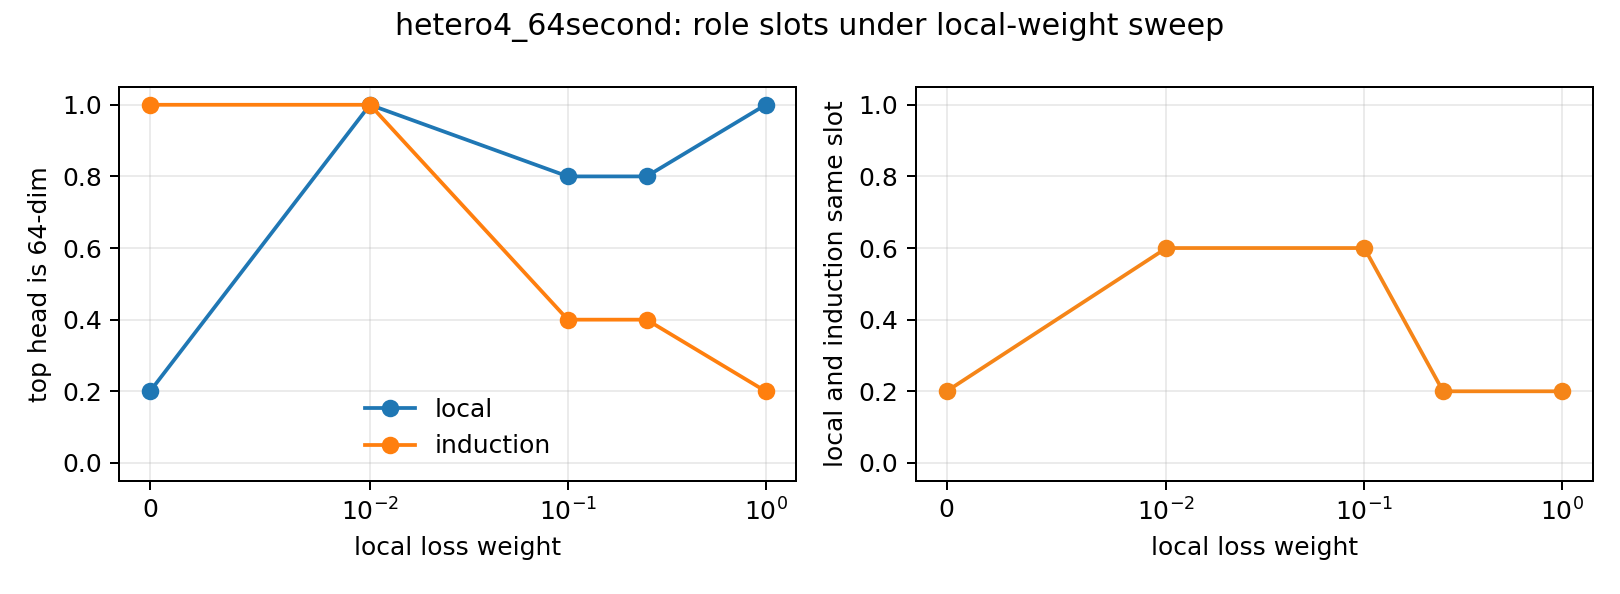
\includegraphics[width=0.88\linewidth]{figures/weight_sweep_top64_and_slot_overlap.png}
  \end{center}
\end{frame}

\begin{frame}{Summary Table}
  \begin{center}
  \scriptsize
  \begin{tabular}{rrrrrr}
    \toprule
    Local weight & Local acc. & Induction acc. & Local top 64 & Induction top 64 & Same slot \\
    \midrule
    0.00 & 0.2264 & 0.9981 & 0.20 & 1.00 & 0.20 \\
    0.01 & 0.9963 & 0.9976 & 1.00 & 1.00 & 0.60 \\
    0.10 & 0.9998 & 0.9976 & 0.80 & 0.40 & 0.60 \\
    0.25 & 0.9999 & 0.9980 & 0.80 & 0.40 & 0.20 \\
    1.00 & 1.0000 & 1.0000 & 1.00 & 0.20 & 0.20 \\
    \bottomrule
  \end{tabular}
  \end{center}

  \vspace{0.7em}
  Induction uses the 64-dim slot when local pressure is absent or tiny, but is
  often displaced once local pressure becomes substantial.
\end{frame}

\begin{frame}{What Changed}
  \textbf{Supported:}
  \begin{itemize}
    \item The [16, 64, 16, 32] layout can put induction on the 64-dim head.
    \item Local pressure changes role allocation among structural slots.
    \item Heterogeneous dimensions create capacity attractors, not fixed semantics.
  \end{itemize}

  \vspace{0.7em}
  \textbf{Nonlinear detail:}
  \begin{itemize}
    \item At local weight 0.01, local learns and both roles use 64-dim heads in 5/5 seeds.
    \item At local weights 0.10, 0.25, and 1.00, induction often moves to 16-dim or 32-dim slots.
  \end{itemize}
\end{frame}

\begin{frame}{Interpretation}
  Best current mechanism:

  \vspace{0.7em}
  \begin{quote}
    Structural heterogeneity creates high-capacity attractor slots; weak task
    pressure can cohabit those slots, while stronger competing pressure can
    displace one role into secondary slots.
  \end{quote}

  \vspace{0.7em}
  This strengthens the architectural-intervention story, but narrows the claim.
  The result is about symmetry breaking, capacity attraction, and task competition,
  not a fixed dimension-to-function semantic taxonomy.
\end{frame}

\begin{frame}{Decision}
  Continue Phase 3 with the capacity-slot competition framing.

  \vspace{0.8em}
  Next decisive tests:
  \begin{enumerate}
    \item Repeat the weight sweep across all four placements of the 64-dim head.
    \item Add a matched-total-dimension condition with two medium-large heads.
    \item Test whether role displacement weakens when there is more than one attractive slot.
  \end{enumerate}

  \vspace{0.7em}
  If those hold, the causal story becomes: heterogeneity breaks permutation
  symmetry, creates capacity attractors, and task pressure allocates roles.
\end{frame}

\begin{frame}{Sources and Provenance}
  \scriptsize
  \begin{itemize}
    \item Report: \texttt{doc/phase3\_toy\_competition\_weight\_sweep.md}
    \item Training script: \texttt{scripts/toy\_competition\_head\_dim\_intervention.py}
    \item Analysis script: \texttt{scripts/analyze\_competition\_weight\_sweep.py}
    \item Run outputs: \texttt{results/phase3\_toy\_competition\_weight\_lw*/}
    \item Combined analysis: \texttt{results/phase3\_toy\_competition\_weight\_sweep/}
    \item Deck data snapshot: \texttt{presentations/2026-05-22-0921-weight-sweep/data/}
  \end{itemize}
\end{frame}

\end{document}
